\documentclass{standalone}
	\usepackage{tikz}
        \graphicspath{ {figures/AM_1_52/} }
	\begin{document}
\begin{tikzpicture}[node distance=0.01cm and 3cm]
 \node[anchor=center] (0) at (0,-0.8) { 1 \ (block1\_conv1) };
\node[anchor=center] at (6,-0.8) { 2 \ (block1\_conv2) };
 \foreach \label [count=\i] in {L0_F5.png,L0_F18.png,L0_F8.png,L0_F23.png,L0_F57.png,L0_F12.png,L0_F41.png,L0_F20.png,L0_F49.png,L0_F59.png,L0_F54.png,L0_F53.png,L0_F48.png,L0_F10.png} { 
 
    \node[draw=none] (\i) at (0,-\i*6em) {\includegraphics[width=0.3\textwidth]{\label} }; 
  }
\node[] (R) at (6,-7.5*6em) {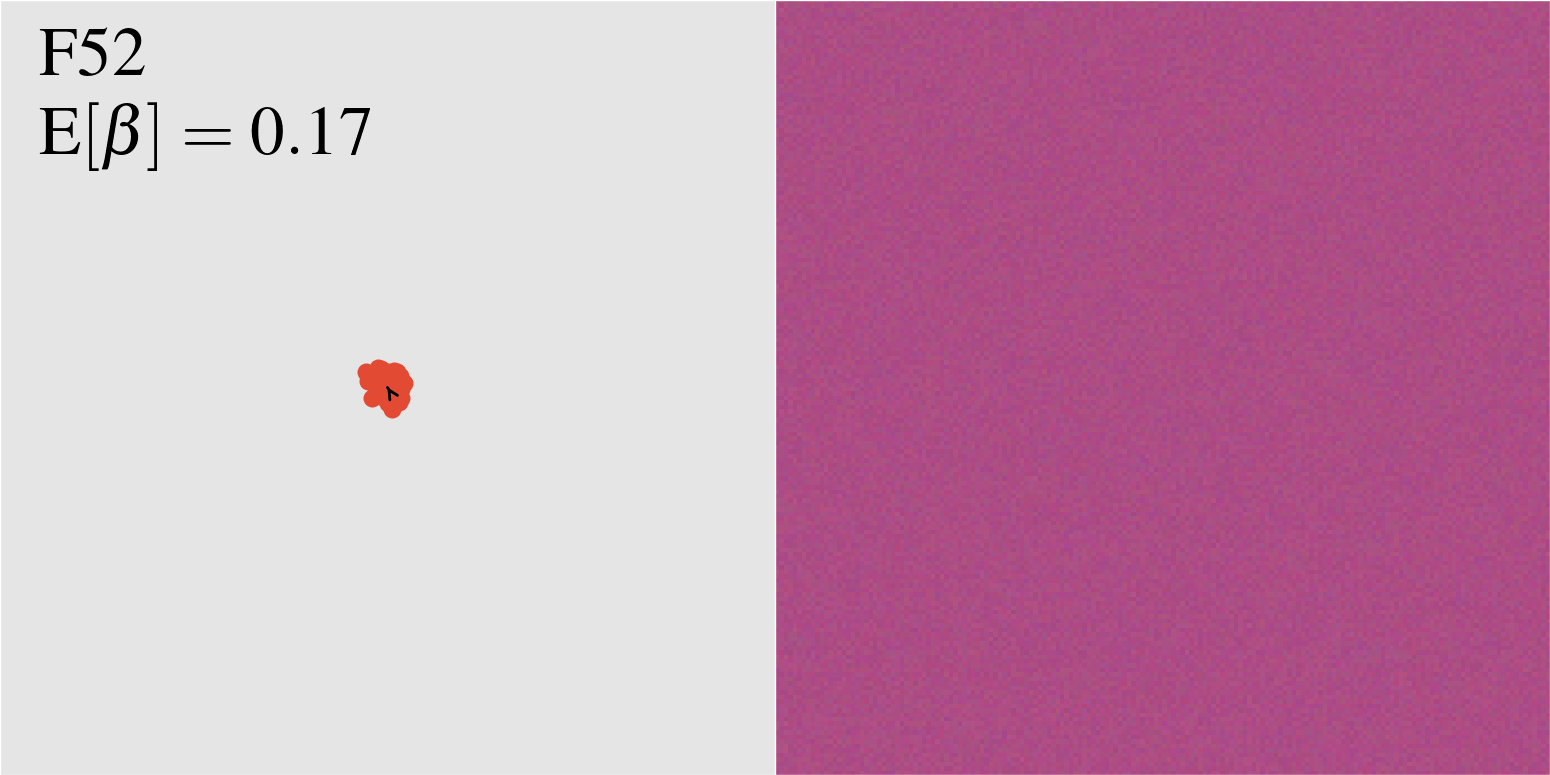
\includegraphics[width=0.3\textwidth]{ L1_F52.png } }; % Adjust the y-coordinate to center
 \draw (1.east) -- (R);
 \draw (2.east) -- (R);
 \draw (3.east) -- (R);
 \draw (4.east) -- (R);
 \draw (5.east) -- (R);
 \draw (6.east) -- (R) node[pos=1, circle, draw, fill=white, minimum size=4pt, inner sep=0pt] {}; 
 \draw (7.east) -- (R);
 \draw (8.east) -- (R);
 \draw (9.east) -- (R);
 \draw (10.east) -- (R) node[pos=1, circle, draw, fill=white, minimum size=4pt, inner sep=0pt] {}; 
 \draw (11.east) -- (R);
 \draw (12.east) -- (R) node[pos=1, circle, draw, fill=white, minimum size=4pt, inner sep=0pt] {}; 
 \draw (13.east) -- (R) node[pos=1, circle, draw, fill=white, minimum size=4pt, inner sep=0pt] {}; 
 \draw (14.east) -- (R);
\end{tikzpicture}
\end{document}
